\documentclass[10pt,journal,compsoc]{IEEEtran}

\newcommand\MYhyperrefoptions{bookmarks=true,bookmarksnumbered=true,
pdfpagemode={UseOutlines},plainpages=false,pdfpagelabels=true,
colorlinks=true,linkcolor={black},citecolor={black},urlcolor={black},
pdftitle={Bare Demo of IEEEtran.cls for Computer Society Journals},%<!CHANGE!
pdfsubject={Typesetting},%<!CHANGE!
pdfauthor={Man-Leong Chan},%<!CHANGE!
pdfkeywords={Computer Society, IEEEtran, journal, LaTeX, paper,
             template}}%<^!CHANGE!


\usepackage{graphicx}
\graphicspath{{res/}{graph/}}
\usepackage{caption}
\usepackage{subcaption}


\begin{document}

\title{Recognising people using body shape analysis}

\author{Man-Leong Chan,~\IEEEmembership{University of Southampton}}

\IEEEtitleabstractindextext{%
\begin{abstract}
We present a combination of 2 methods for analysing a person's body shape and ultimately attempt to identify subjects from a set of photos by recognision. Silhouette and limb position analysis provides us metrics of the person's standing posture, which is used in our recongition algorithm. 
\end{abstract}

% Note that keywords are not normally used for peerreview papers.
}


% make the title area
\maketitle
\IEEEdisplaynontitleabstractindextext
\IEEEpeerreviewmaketitle



\section{Introduction}

Given a set of images each with a subject standing in front of a green screen with one facing forward and another facing sideways, we can recongnise a person's body shape and attempt to identify them individually. This involve extracting the subject from an image, generating subject's metrics and finally identification.  




\section{Image processing}

\subsection{Green screen and background removal}
Our domain is a set of photos each with a subject in front of a green screen standing on a treadmill. Subject extraction requires the removal of the green screen as well as any background captured outside of the green screen area. Couple of samples of green screen color reveals the average screen color to be \textit{rgb(56, 175, 93)}. Image area beyond the green screen area is cropped to remove excess background area. 

\begin{figure}[!htb]
\begin{subfigure}[h]{0.3\linewidth}
    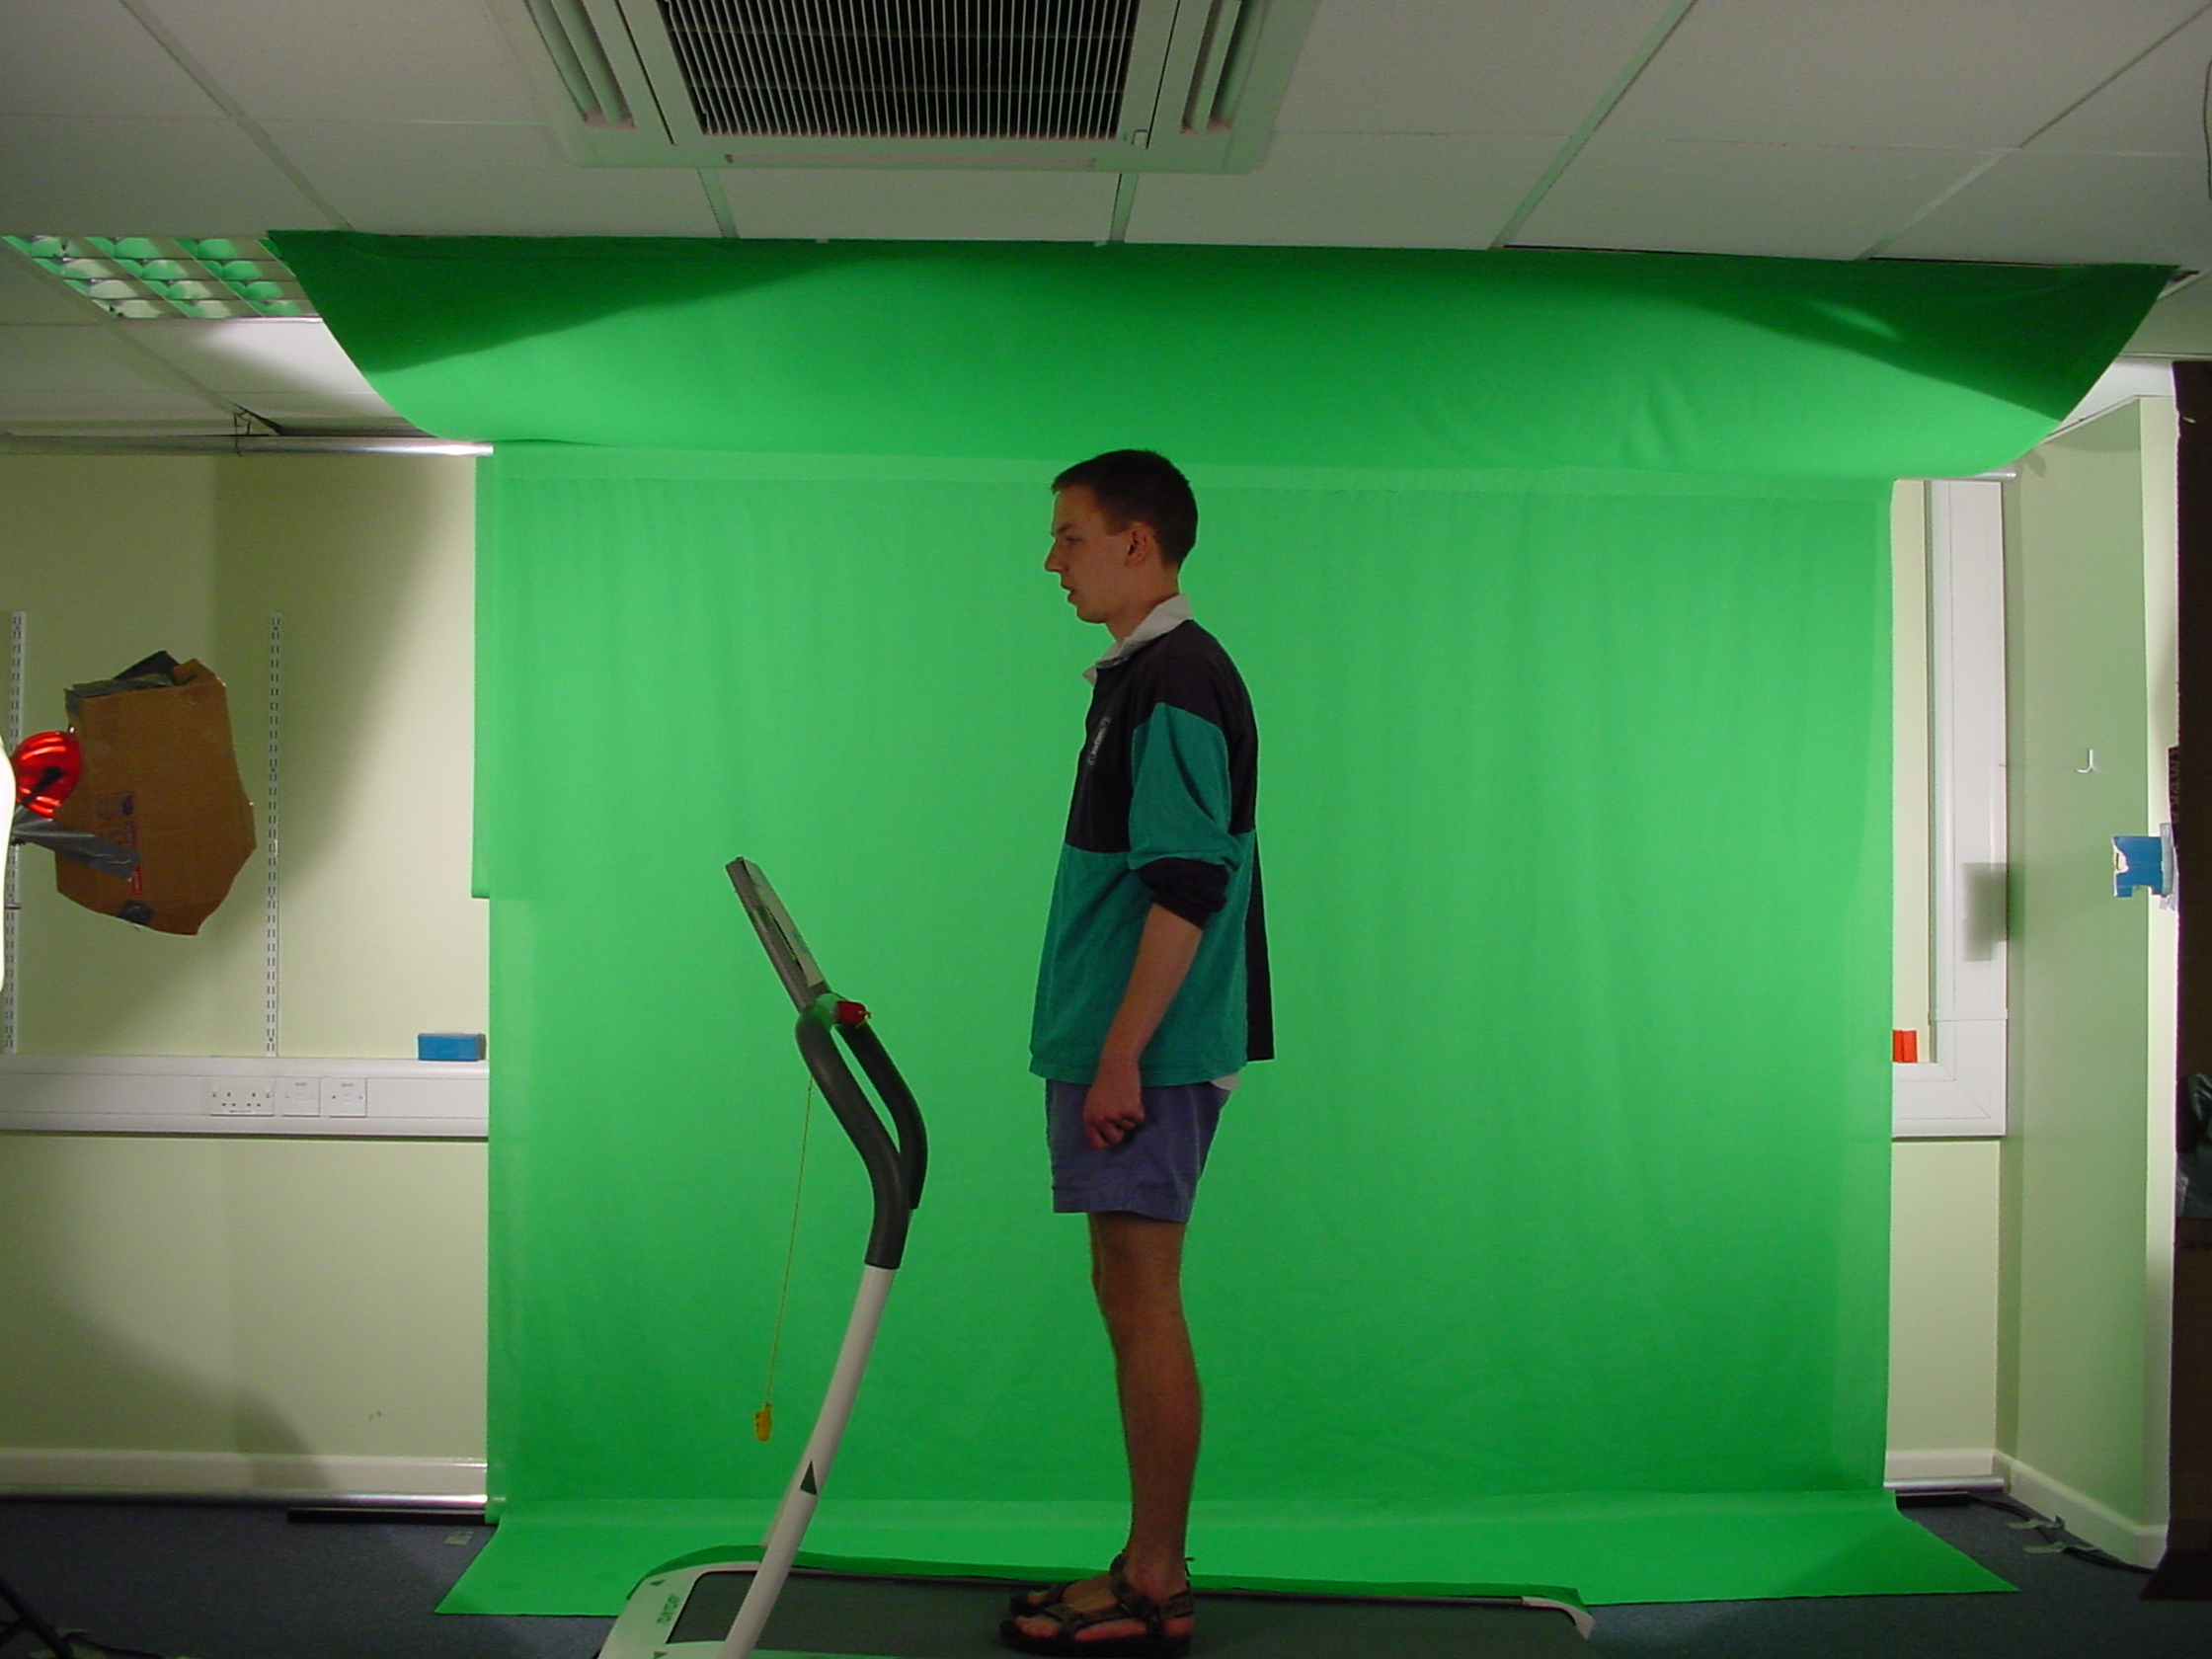
\includegraphics[width=\linewidth]{original}
\caption{Original}
\end{subfigure}
\hfill
\begin{subfigure}[h]{0.3\linewidth}
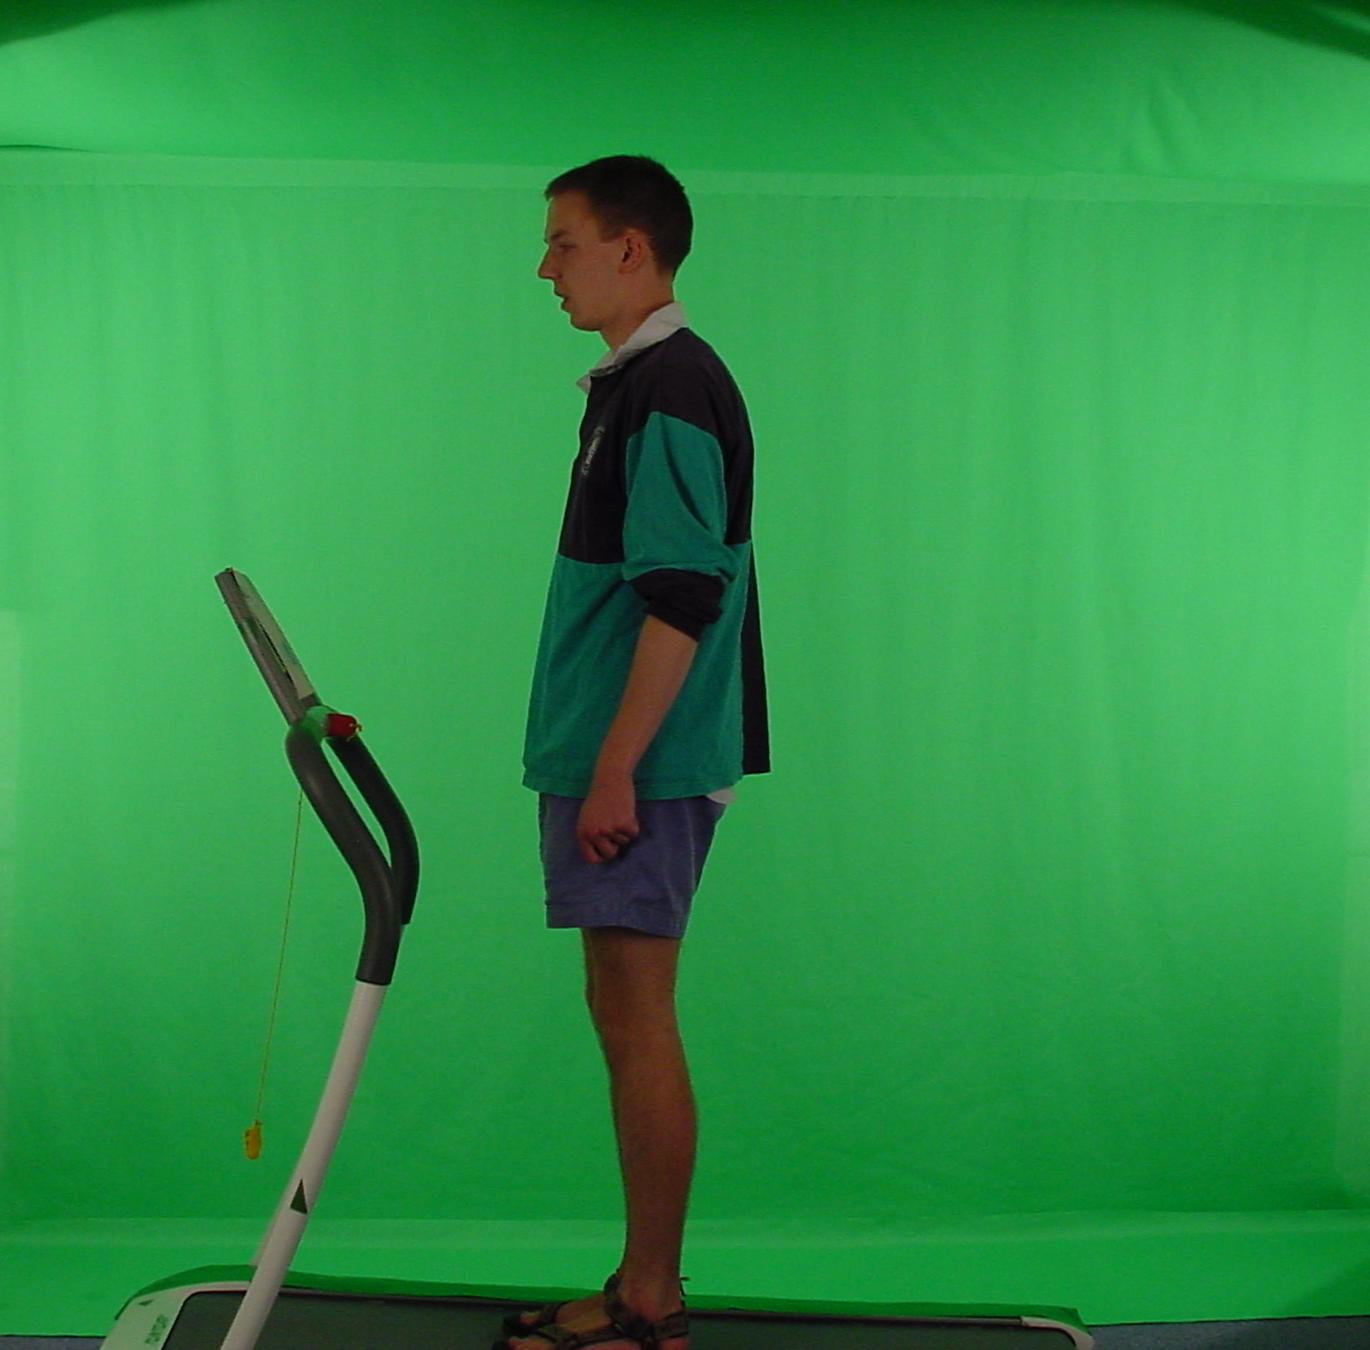
\includegraphics[width=\linewidth]{cropped}
\caption{Cropped}
\end{subfigure}
\hfill
\begin{subfigure}[h]{0.3\linewidth}
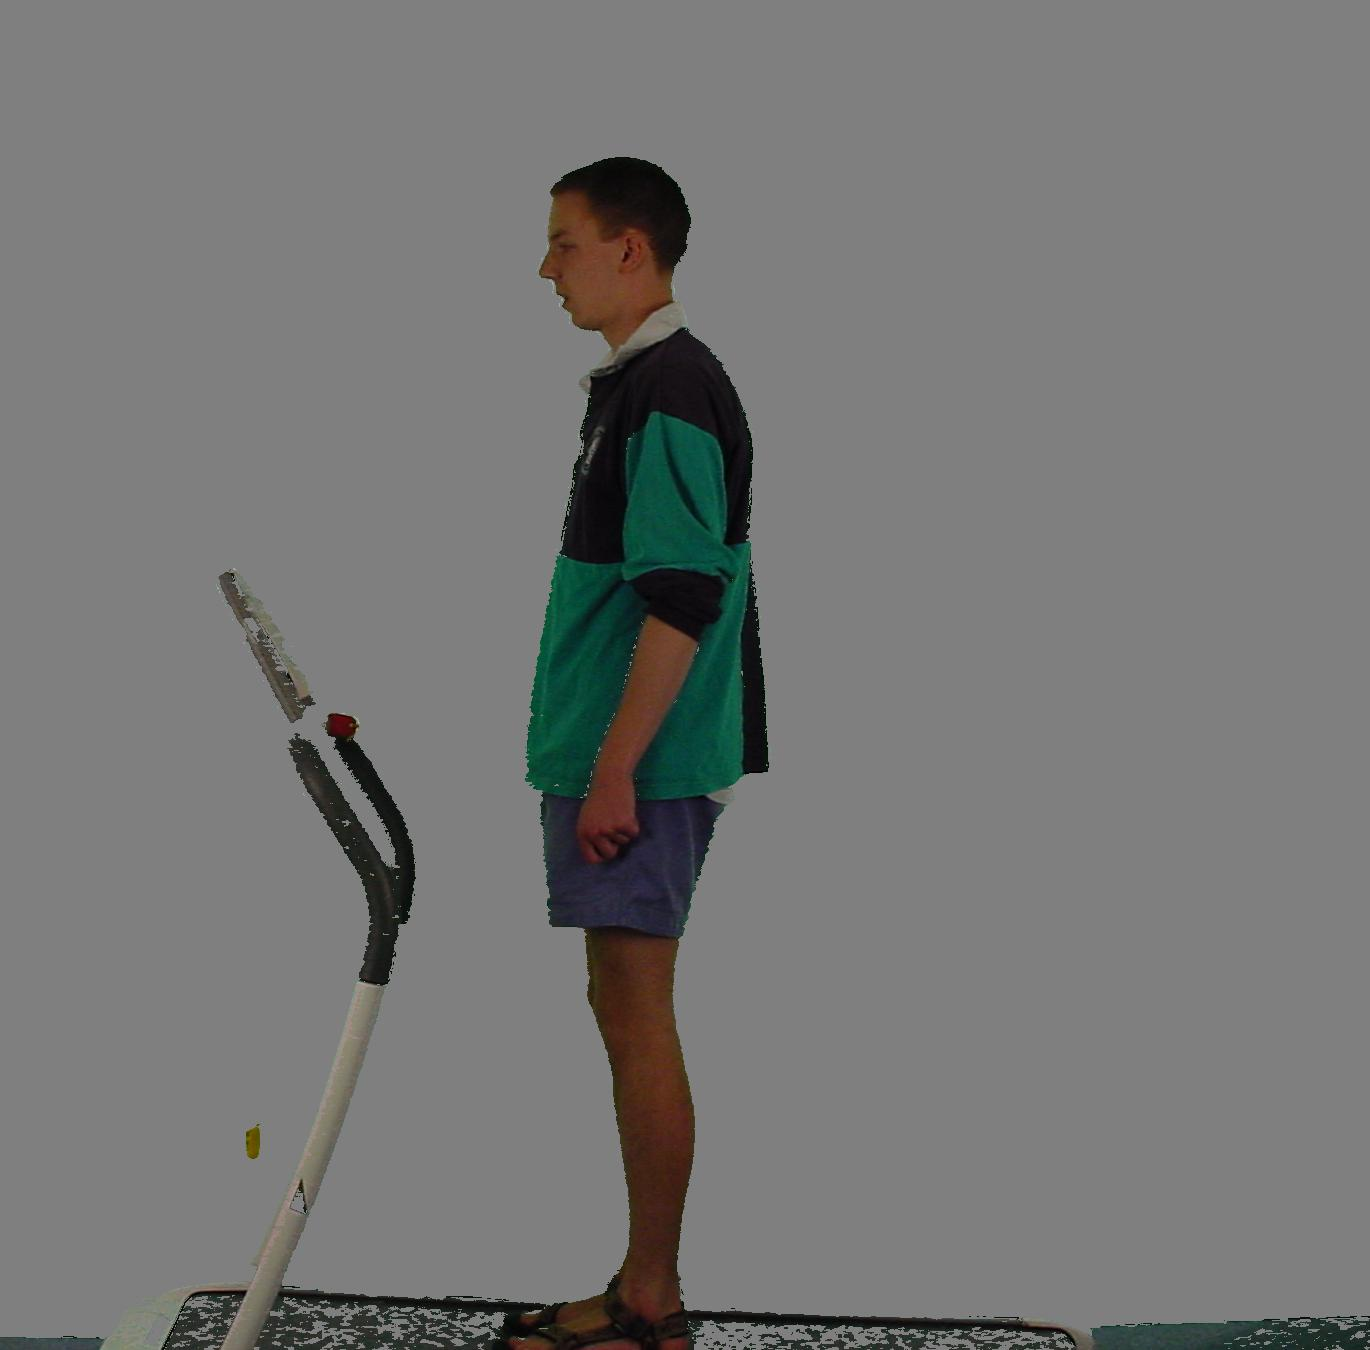
\includegraphics[width=\linewidth]{noGreen}
    \caption{bg removed}
\end{subfigure}%
\caption{Background removal}
\end{figure}


\subsection{Skin tone extraction}
Subject's limbs were extracted according to their skin tone. This extraction was done by analysing the HSV value of every pixel in the image. Where 0 \textless\textit{Hue} \textless25, 0.50 \textless\textit{Saturation} \textless0.98 and \textit{Value} \textgreater0.22. Our hue control selected skin tone from a range of color angles, it allowed the algorithm to be inclusive with a range of skin colour of different race and background\cite{Kolkur2017}. Saturation controled the range of colour sharpness which was crucial for our algorithm to differentiate between skin colour and shadows. The subject's skin surface under a reasonably well litted environment would have a higher saturation value than clothing in beige or brown.

\begin{figure}[!htb]
\begin{subfigure}[h]{0.45\linewidth}
    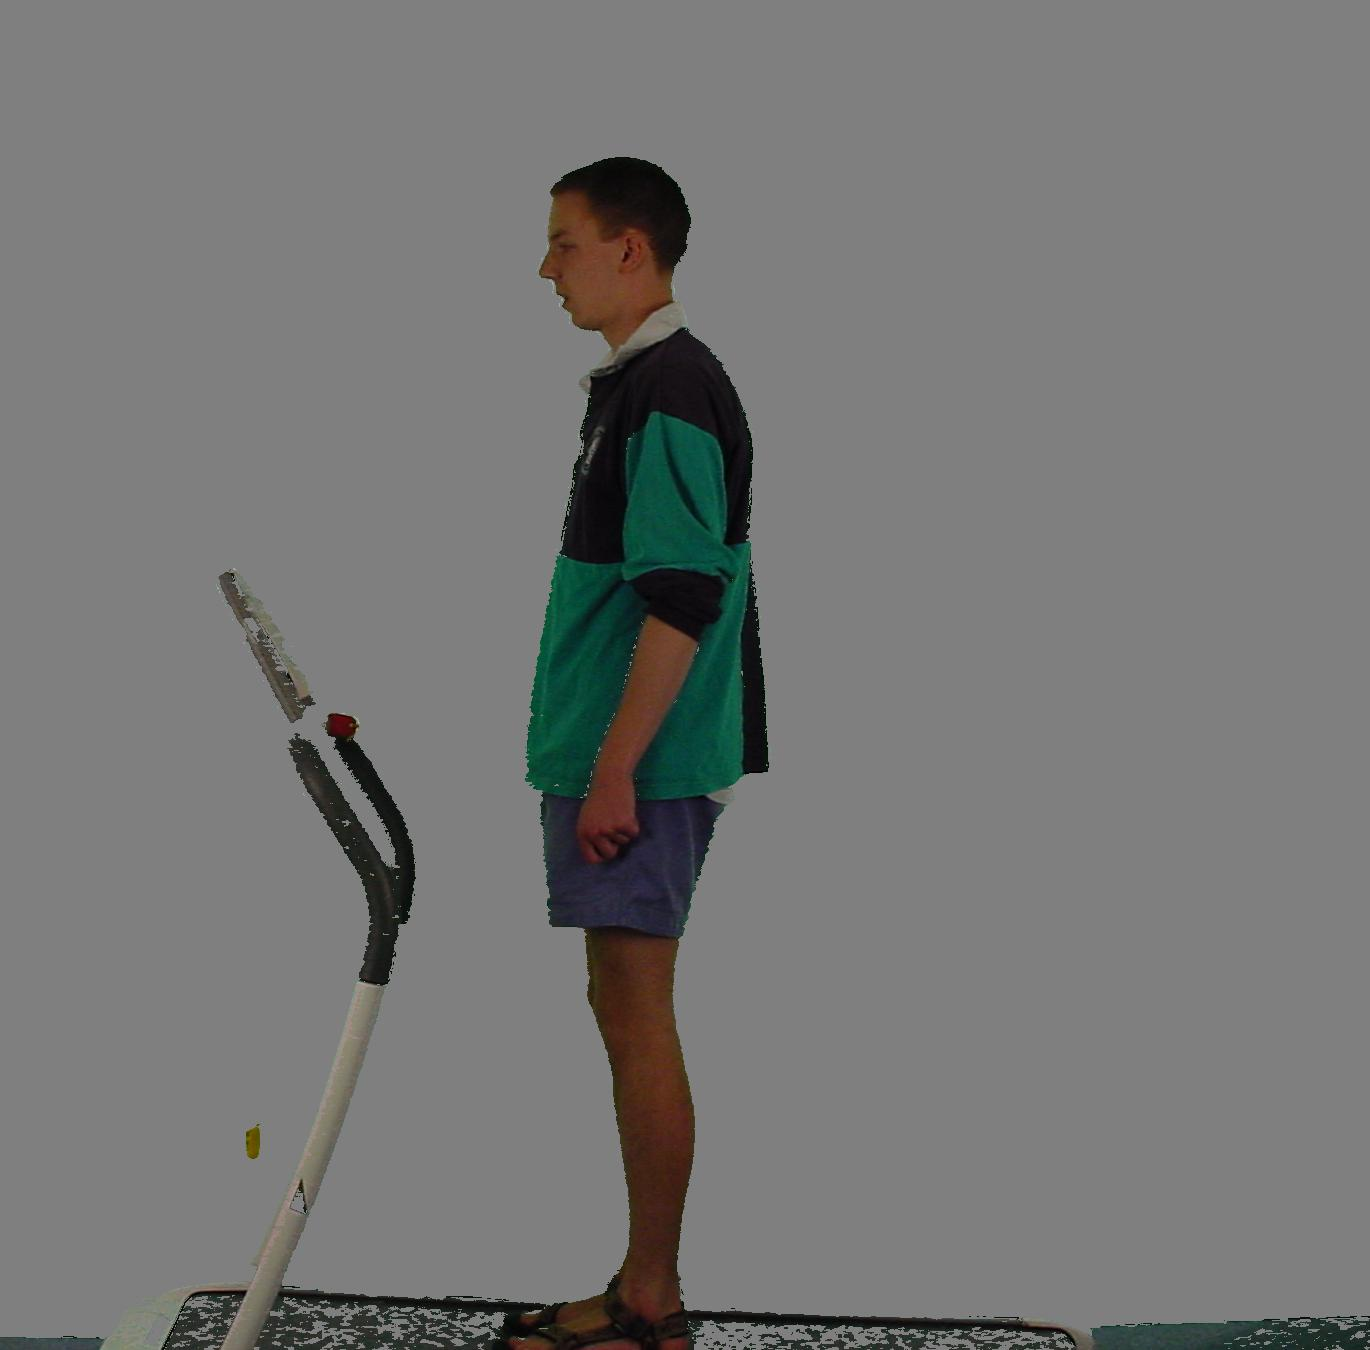
\includegraphics[width=\linewidth]{noGreen}
\caption{Before extraction}
\end{subfigure}
\hfill
\begin{subfigure}[h]{0.45\linewidth}
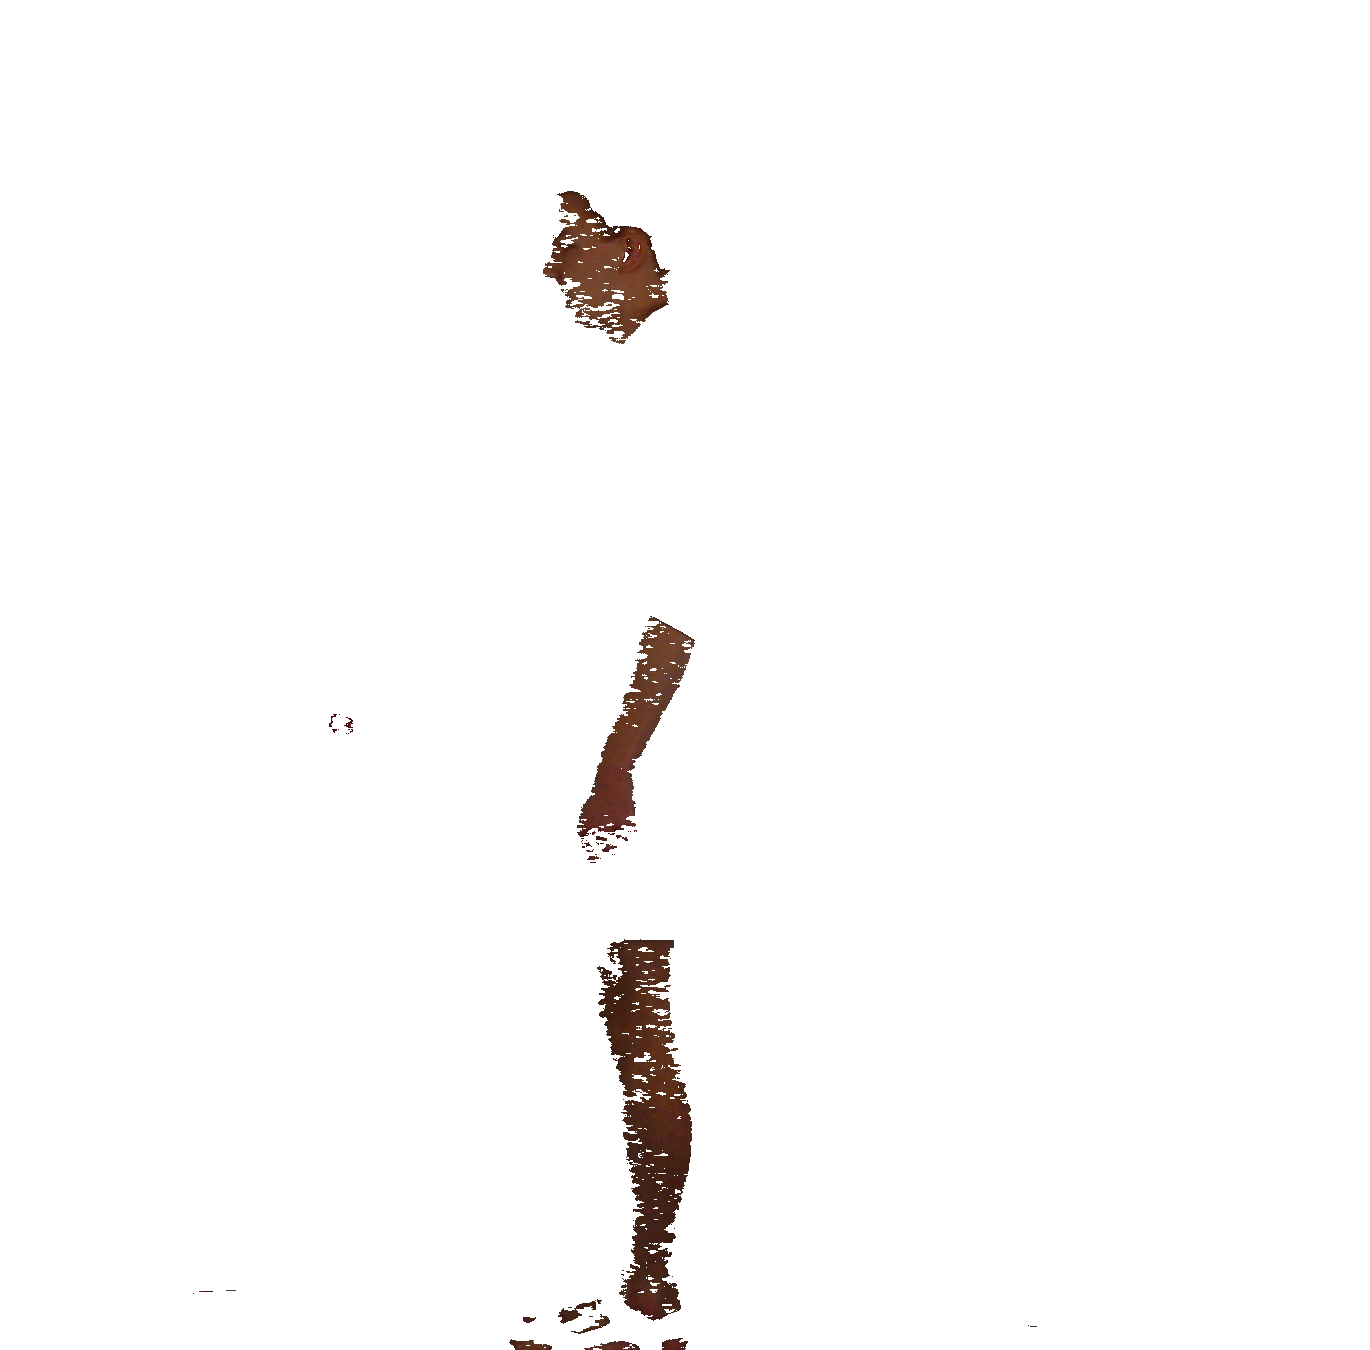
\includegraphics[width=\linewidth]{skin}
\caption{After extraction}
\end{subfigure}%
\caption{Skin tone extracton by HSV}
\end{figure}

Obviously tone extraction obviously relied on the subject exposing some part of their body. Primarily it required the subject to expose their face and hand for the best outcome. Therefore we are assuming that our subject does not wear a Niqab or gloves. 


\subsection{Limb Segmentation}
Skin tone extraction gave us many fragments of skin color in different sizes. The larger fragments gave us more interesting ideas on what those limbs could be, where as the smaller fragments scattered across the image could be noise which so happened to have the same HSV values as our subject's skin.\cite{Marvin}
\\ \\
In order to carry out further analysis, we had to outline our desired fragments which were potentially part of subject's limbs. A floodfill analysis was used to determine the outline of those potential targets. It determined fragments which were connected in this 2 dimentional pixel array and output the outline of each fragments. Fragments which are smaller than any desired features were ignored to reduce noise in the data. 
\\ \\
Once the fragments were identified, they were subjected to feature analysis. Up to this point, the fragments are nothing but scattered data, feature analysis aims to identify which body part these fragments belong and this would give us useful data towards analysing subject's standing posture. Here we made a couple of assumption. 
\begin{itemize}
    \item Firstly the subject is not raising their hands above their head at the moment when the picture was taken. 
    \item Secondly the subject is not vertically rotated. 
\end{itemize}
Then we ran a verticle analysis where we first identify the person's head followed by their arms and leg. We assumed not everyone were wearing short and exposing the skin from their legs, so identifying legs were not compulsory. Similarly, some subjects were wearing long-sleeves and others were wearing t-shirts, the variation between the detected limb size were accounted for.


\begin{figure}[!htb]
\centering
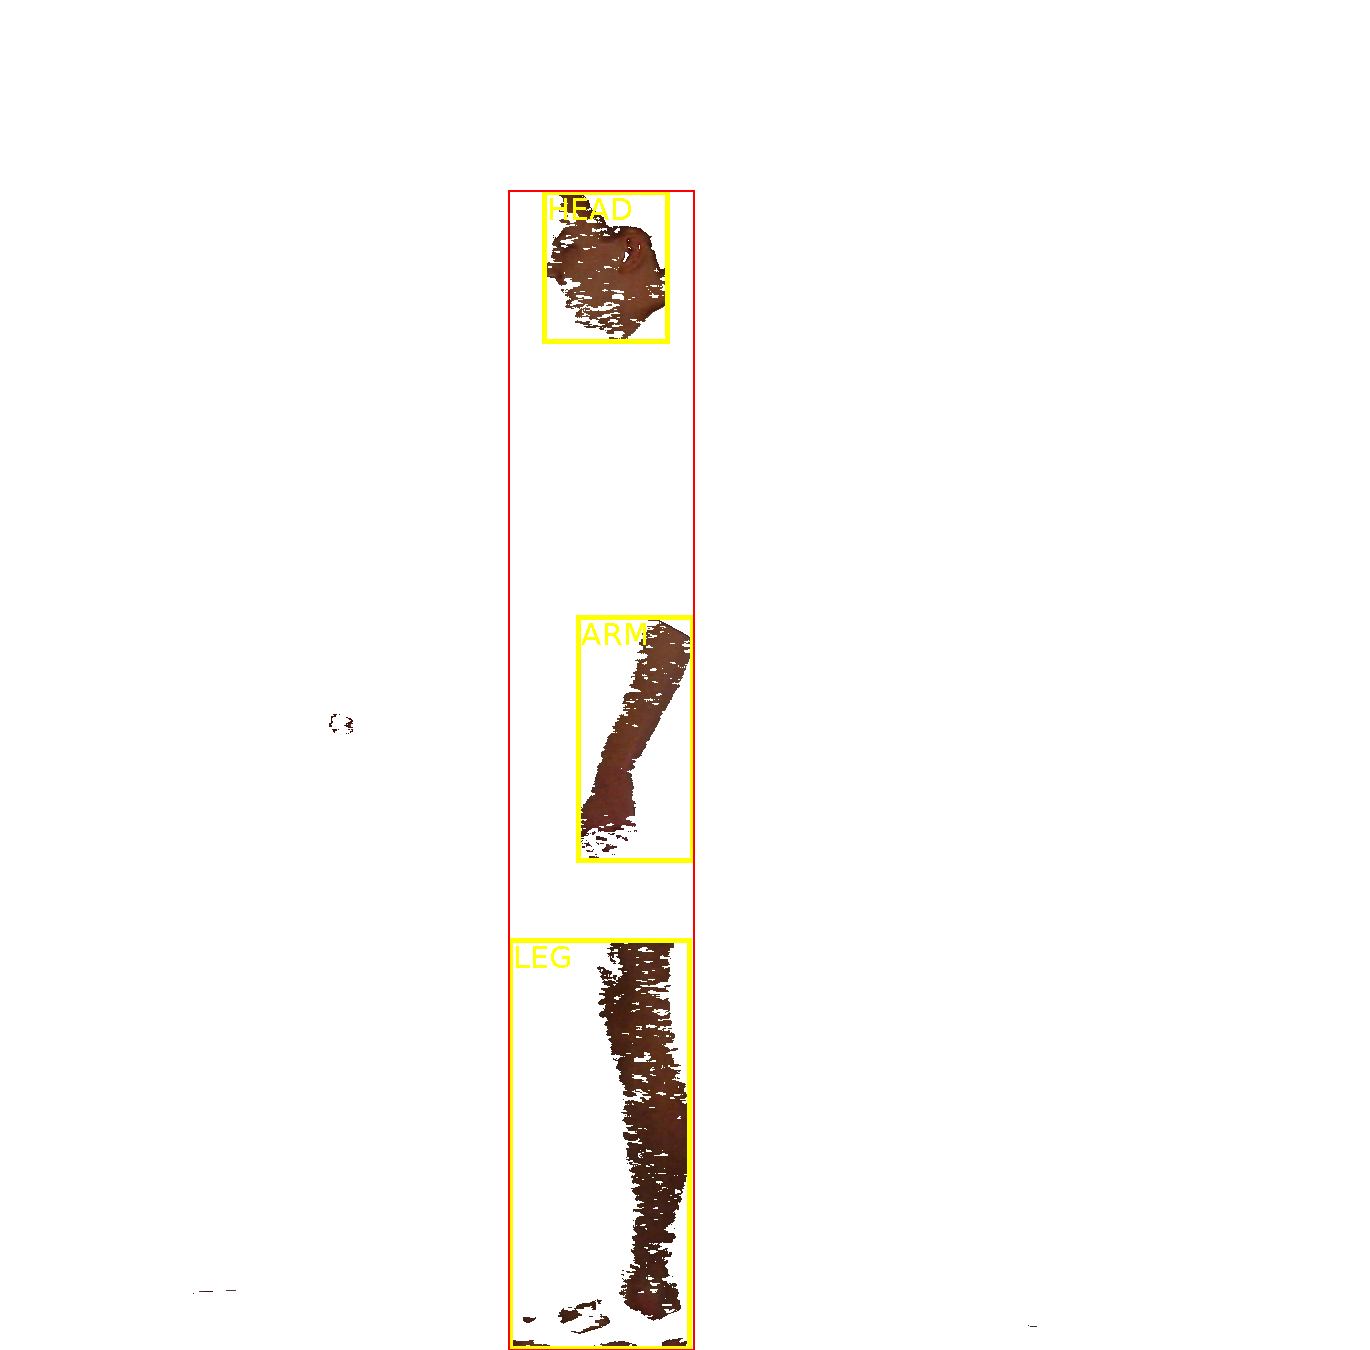
\includegraphics[width=0.7\linewidth]{segment_analysis}
\caption{Limb identification}
\end{figure}

\subsubsection{Statistics}
Accuracy of limb identification

\begin{center}
 \begin{tabular}{||l | l||} 
 \hline
 Total number of images &  112 \\ 
 \hline
 Number of limbs identified & 391 \\ 
 \hline
 False negatives & 8 \\
 \hline
 False positives & 25 \\
 \hline
 Error rate & 8.4\% \\
 \hline
\end{tabular}
\end{center}


\subsection{Silhouette extraction}
Edge detection technique was used to extract the subject's silhouette. All three common edge detection technique - Sobel, Roberts, Susan was tested ultimately Roberts' provided the cleanest results. Sobel gave us some vibrant lines but it contained too much redundent data of the treadmill.
\\ \\
The result of Roberts' were able to outline our subject and some of the treadmill. We used the parimeters of our limb segmentation to estimate our subject's location and ignored edges which were far away from the subject.

\begin{figure}[!htb]
\centering
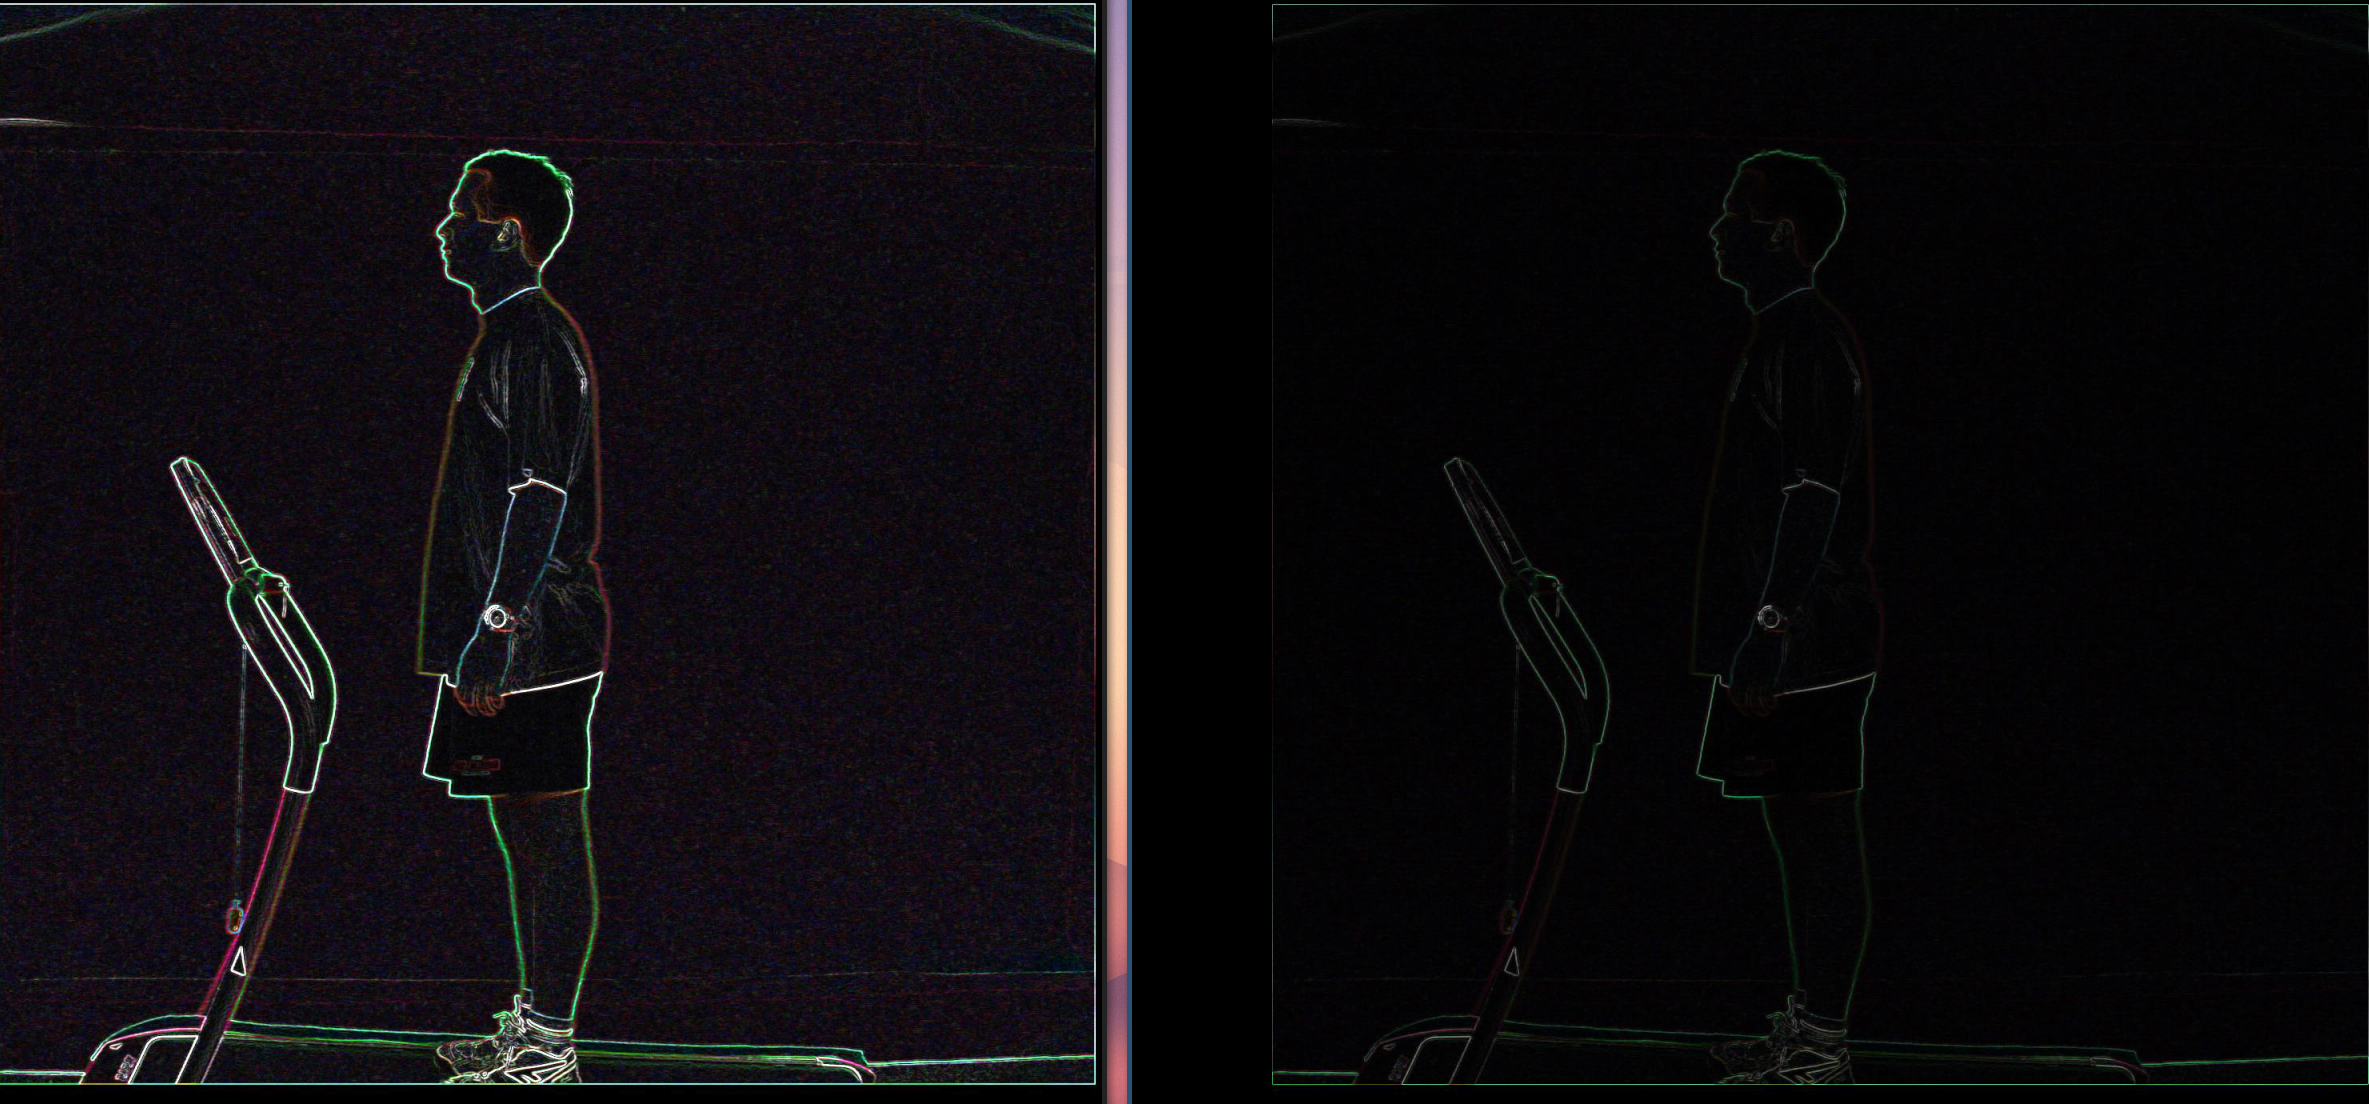
\includegraphics[width=0.7\linewidth]{edgeDetectionComp}
    \caption{Edge detection: Sobel (left) vs Roberts (right)}
\end{figure}

\subsection{Results}
The end result of both limb analysis and silhouette extraction has allowed us to gain a lot of metrics for further analysis into the subject's body shape as well as standing posture.

\begin{figure}[!htb]
\centering
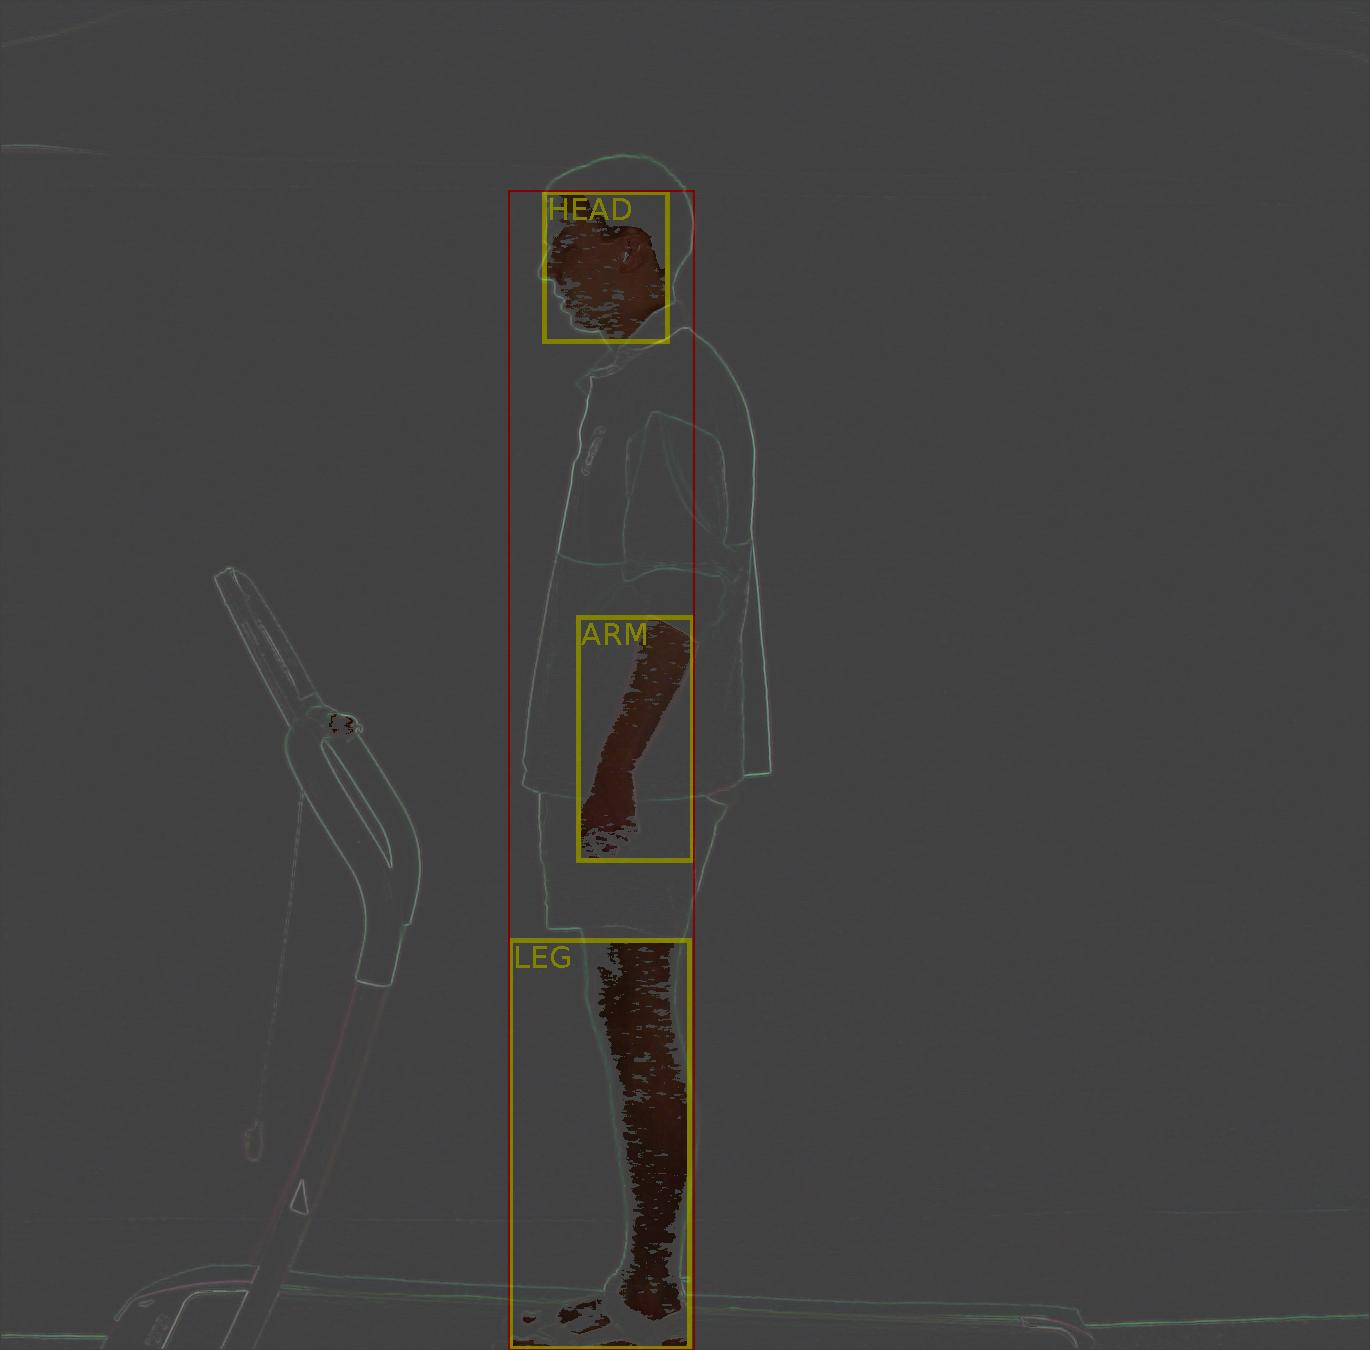
\includegraphics[width=0.7\linewidth]{combined}
    \caption{Silhouette with limb analysis}
\end{figure}

Positional data of each subject including their limbs were stored in a seperate JSON file to aid subject identification in later parts.



\section{Subject identification}


\subsection{Domain}

\subsubsection{Silouette data}
From our silhouette extraction, we can measure the width of a subject and occationally the height of the subject. A simple metric that we can measure is the surface area of the person, obviously this is not a great idea as the subject's surface area depends on how close the subject is standing (scaling problem). A better idea was to calculate the ratio of height against their width. This can give us a brief estimate of the person's body ratio, in other words if the person is short and
wide or tall and skinny. However we could not assume this measurement was always available. The noise generated from the bottom of the image did not allow us to collect reliable information of the subject's feet, therefore we cannot accurately determine the subject's height. One way to get around the problem is to uniformly measure each subject to the lowest point of their leg. This on the other hand struggles from inconsistancy between subject wearing trousers and shorts, which affects if
the lower limb data is available. Nevertheless, this data is used whenever available during our identification phase.

\begin{figure}[!htb]
\centering
\includegraphics[width=0.7\linewidth]{heightWideRatio}
    \caption{Silouette identification analysis}
\end{figure}


\subsubsection{Front facing limb analysis}
Instead of analysing the ratio between the subject's height and width, limb positional analysis provides much better results. We compared two main metrics when applicable.

\begin{itemize}
    \item horizontal position of where the head is relative to their arms. Everyone has a slightly different standing posture, this determines if one of your arm is extending further than the other. 
    \item the top position of the arm area. Again, depending on the subject's standing posture, one of their arm is naturally raised higher than the other. \cite{Mittal2011}
\end{itemize}

\begin{figure}
    \centering
    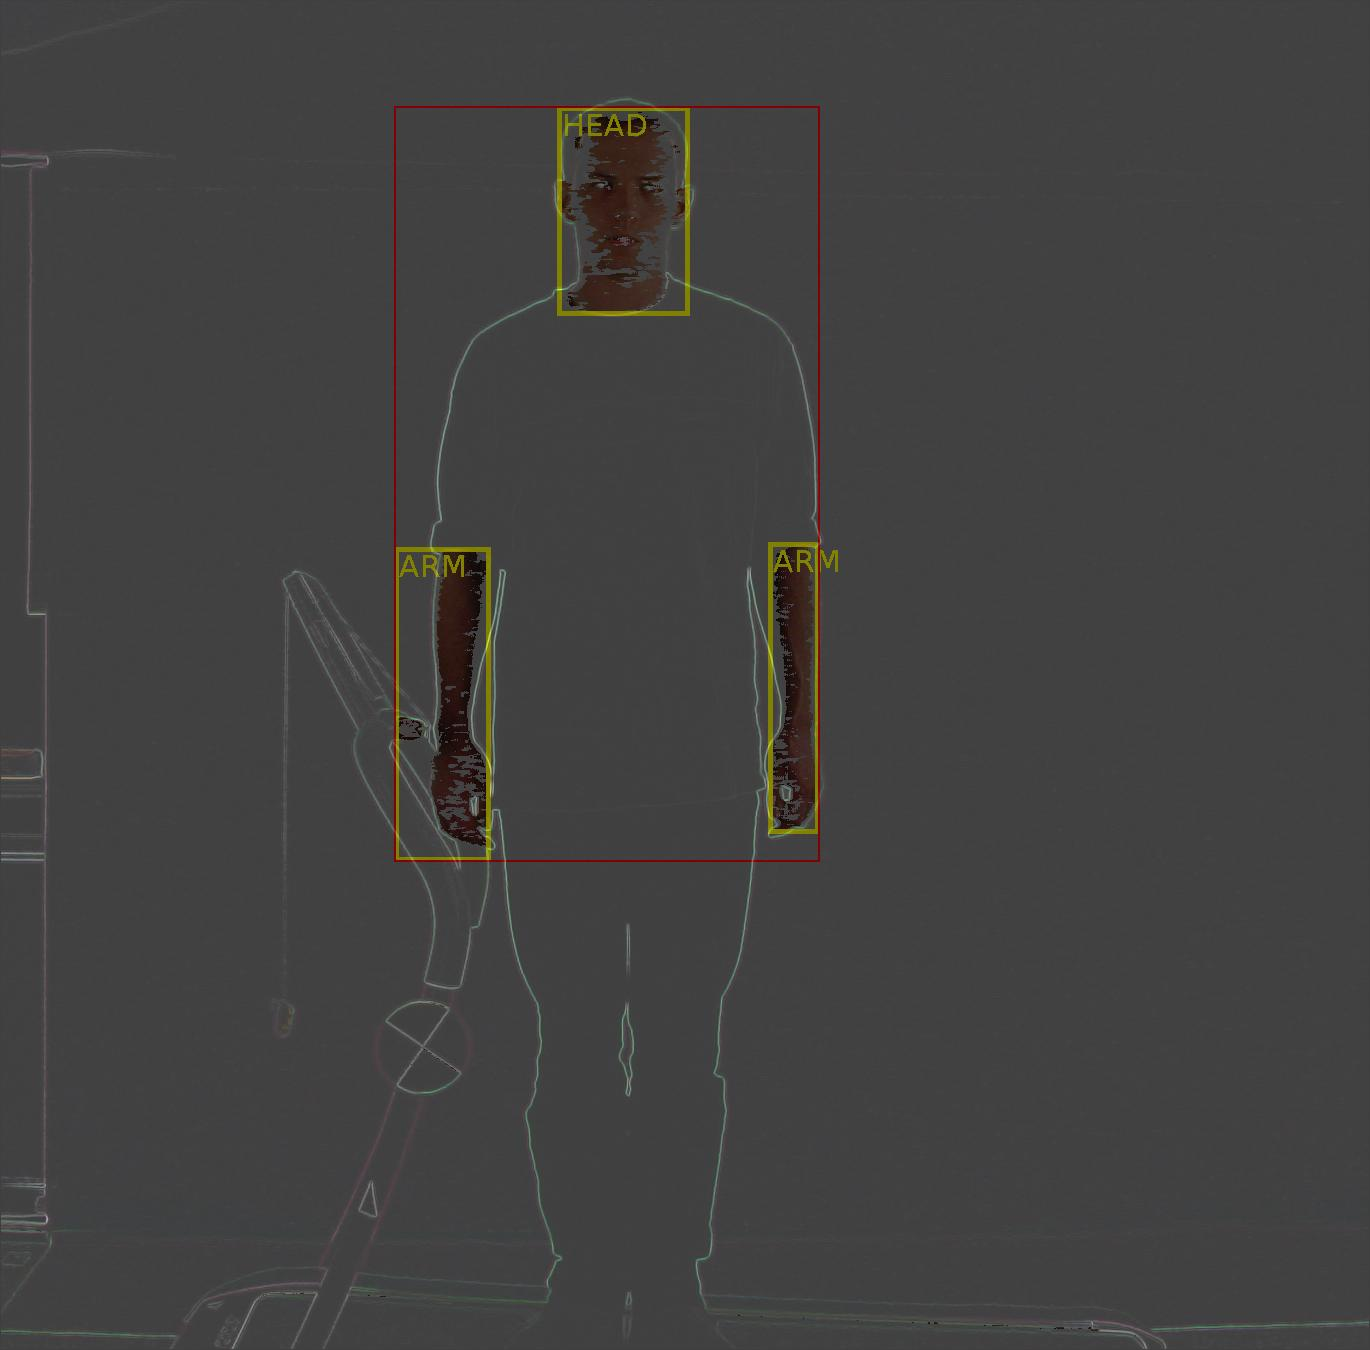
\includegraphics[width=0.8\linewidth]{frontFacing}
    \caption{Height difference of 5px between subject's arm}
\end{figure}

The diagram below demonstrate the head position being a better metrics than height-width ratio as there is no error bar involved. The image has been scaled by 25-times its original size for visual purposes.

\begin{figure}
\centering
\includegraphics[width=1\linewidth]{front1}
    \caption{Head position relative to arm (mid-points)}
\end{figure}

After experimenting with vertical positional difference between arms, we discovered the maximum detected difference is only 12 pixel apart, therefore unsuitable for subject identification.




\subsubsection{Side facing limb analysis}
Side facing image analysis overall had much better results than front facing images, 51 out of 52 images identified all limbs correctly. This allowed us to run analysis with extra confidence. We utilize the back of the subject arm and compared to the position of the subject's head. This measures of how much hunch the subject has in a up right position. 

\begin{figure}
\centering
\includegraphics[width=1\linewidth]{headPosition}
    \caption{Side view head position relative to the back of the arm}
\end{figure}


\section{Conclusion}
Limb extraction gave us very interesting metrics for measuring a person's standing posture and it has significant advantages compared to pure silouette analysis. While silouette analysis heavily rely on the camera's position, limb extraction provided very useful additional data to aid recognition analysis. Given the quality of the images, our algorithm still manages to extract the subject with reasonable reliability, and this signals the possibility of this approach in the future.



\bibliographystyle{plain}
\bibliography{bibtex}

\end{document}



